
% ----------------------------------------------------------------------
\introduction
\label{sec:intro}
% ----------------------------------------------------------------------

\begin{figure}[t]
	\vspace*{2mm}
	\begin{center}
		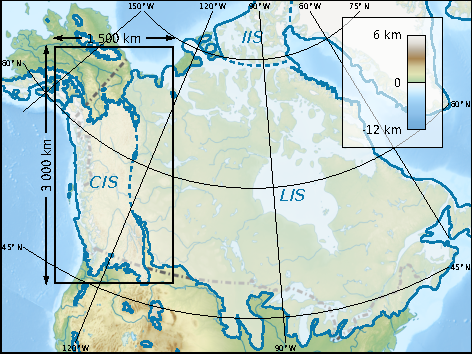
\includegraphics[width=8cm]{cordillera-climate-locmap}
	\end{center}
	\todo[inline, color=cyan]{Reference needed. I have to figure out where the ice sheet's outline comes from. I got it from Martin who got it from Sarah who, I think, got it from Johan, who...}
	\caption{Shaded relief map of northern North America. The frame delimits the modelling domain. After ETOPO1 \citep{data:etopo1} and Natural Earth Data \citep{data:naturalearth}.}
	\label{fig:locmap}
\end{figure}

\emph{Coming soon...}

